%%
%% This is file `sample-authordraft.tex',
%% generated with the docstrip utility.
%%
%% The original source files were:
%%
%% samples.dtx  (with options: `authordraft')
%% 
%% IMPORTANT NOTICE:
%% 
%% For the copyright see the source file.
%% 
%% Any modified versions of this file must be renamed
%% with new filenames distinct from sample-authordraft.tex.
%% 
%% For distribution of the original source see the terms
%% for copying and modification in the file samples.dtx.
%% 
%% This generated file may be distributed as long as the
%% original source files, as listed above, are part of the
%% same distribution. (The sources need not necessarily be
%% in the same archive or directory.)
%%
%% The first command in your LaTeX source must be the \documentclass command.
\documentclass[sigchi]{acmart}

%% For page numbers! Yay!
\settopmatter{printfolios=true}

%%
%% Remove the ACM copyright information. Found on:
%% https://tex.stackexchange.com/questions/346292/how-to-remove-conference-information-from-the-acm-2017-sigconf-template
% Removes citation information below abstract
\settopmatter{printacmref=false}
% removes footnote with conference information in first column
\renewcommand\footnotetextcopyrightpermission[1]{} 

%% Please use this for your title. We use the long version for the title on the
%% first page and the shorter version for the running page header on the right.
\newcommand{\myLongTitle}{My Long Title of my Essay} %% @TODO
\newcommand{\myShortTitle}{Short Title of Essay} %% @TODO

%% NOTE that a single column version may be required for 
%% submission and peer review. This can be done by changing
%% the \doucmentclass[...]{acmart} in this template to 
%% \documentclass[manuscript,screen,review]{acmart}
%% 
%% To ensure 100% compatibility, please check the white list of
%% approved LaTeX packages to be used with the Master Article Template at
%% https://www.acm.org/publications/taps/whitelist-of-latex-packages 
%% before creating your document. The white list page provides 
%% information on how to submit additional LaTeX packages for 
%% review and adoption.
%% Fonts used in the template cannot be substituted; margin 
%% adjustments are not allowed.
%%
%% \BibTeX command to typeset BibTeX logo in the docs
\AtBeginDocument{%
  \providecommand\BibTeX{{%
    \normalfont B\kern-0.5em{\scshape i\kern-0.25em b}\kern-0.8em\TeX}}}

%%
%% Remove copyright note by ACM: Found on:
%% https://tex.stackexchange.com/questions/21536/how-to-remove-the-copyright-box-on-a-paper-that-uses-the-acm-sig-alternate-cls-c
\setcopyright{none} 

%%
%% end of the preamble, start of the body of the document source.
\begin{document}

%%
%% The "title" command will get the content of "myLongTitle".
\title{\myLongTitle{}}

%% The "subtitle" command is used for the course title and will change
%% every semester.
\subtitle{Proseminar "Interactive Intelligent Systems", Winter Term, 2020/21}

%%
%% The "author" command and its associated commands are used to define
%% the author and affiliation.
\author{Firstname Lastname} %% @TODO
\affiliation{%
  \institution{Freie Universität Berlin}
  \city{Berlin}
  \country{Germany}
}
\email{firstname.lastname@fu-berlin.de} %% @TODO

%%
%% By default, the author name and the "short title" of the document is
%% printed in the page headers. As the full name and the title is sometime very
%% long and stuff might overlap, please use a short version of your name here.
\renewcommand{\shortauthors}{F. Lastname - \myShortTitle{}} %% @TODO

%%
%% This snippet is used a the page header on the outer. This should be changes
%% every semester.
\acmConference[Proseminar "Interactive Intelligent Systems"]{PS IIS}{Winter Term}{2020/21}

%%
%% The abstract is a short summary of the work to be presented in the
%% article.
\begin{abstract}
  Lorem ipsum dolor sit amet, consectetur adipiscing elit, sed do eiusmod tempor incididunt ut labore et dolore magna aliqua. Ut enim ad minim veniam, quis nostrud exercitation ullamco laboris nisi ut aliquip ex ea commodo consequat. Duis aute irure dolor in reprehenderit in voluptate velit esse cillum dolore eu fugiat nulla pariatur.
\end{abstract}

%%
%% Keywords. The author(s) should pick words that accurately describe
%% the work being presented. Separate the keywords with commas.
\keywords{please, add, your, keywords, here}

%% A "teaser" image appears between the author and affiliation
%% information and the body of the document, and typically spans the
%% page.
%% This image is optional, please remove it of you dont need it!
\begin{teaserfigure}
  
\includegraphics[width=\textwidth]{sampleteaser}
  \caption{Some Caption below the figure.}
  \Description{Some description, you need it because.}
  \label{fig:teaser}
\end{teaserfigure}

%%
%% This command processes the author and affiliation and title
%% information and builds the first part of the formatted document.
\maketitle

\pagenumbering{arabic}

%%
%% Add a table of contents to this ACM template
%% Removed "Abstract", "ACK", and "References" from TOC (2401 in acmart.cls)
%% Removing the Contents headline from the TOC!
\let\oldaddcontentsline\addcontentsline
\newcommand{\stoptocentries}{\renewcommand{\addcontentsline}[3]{}}
\newcommand{\starttocentries}{\let\addcontentsline\oldaddcontentsline}

\stoptocentries% Stop adding content to the ToC
\tableofcontents
\starttocentries% Resume adding content to the ToC

\section{Introduction}
This \LaTeX\ template should be used for all seminars at Human-centered Computing\footnote{\url{https://www.mi.fu-berlin.de/en/inf/groups/hcc/index.html}}. This template is a slightly modified version of the \emph{ACM Conference Proceedings "Master" Template}.\footnote{Downloaded at \url{https://www.overleaf.com/latex/templates/acm-conference-proceedings-master-template/pnrfvrrdbfwt} on December 21st, 2020} The ``\verb|acmart|'' document class is used. The template style is ``\verb|sigchi|'' with no additional parameters. Please use the template as it is. There is no need of changing the typeface, spacing or any other layout elements. Especially please do not use ``\verb|\vspace{}|'' or ``\verb|\hspace{}|'' commands.


\section{Title Information}
The title of your work should use capital letters appropriately -
\url{https://capitalizemytitle.com/} has useful rules for
capitalization. There is a long version of your title {\verb|\newcommand{\myLongTitle}|} and a short version {\verb|\newcommand{\myShortTitle}|}. The long version is used on the first page. The short version is used in the page headers. Please provide both versions. The subtitle is usually predefined and set to the name of this seminar. Do not insert line breaks in your title.

\section{Authors and Affiliations}
Please add your author information. This includes your
\emph{firstname}, \emph{lastname}, and \emph{e-mail}. Also add your name to the 
\verb|shortauthors| command and abbreviating your first name. This will display your name together with your short title on the top right page header and the shorter version will prevent overlapping text.

\section{Rights Information}
All ACM copyright information is removed from this template. Please refer the the comments on how this was done.

\section{User-Defined Keywords}
User-defined keywords are a comma-separated list of words and phrases
of the authors' choosing, providing a more flexible way of describing
the work presented. Please add your keywords below the abstract.

\section{Sectioning Commands}
Your work should use standard \LaTeX\ sectioning commands:
\verb|section|, \verb|subsection|, \verb|subsubsection|, and
\verb|paragraph|. They should be numbered; do not remove the numbering
from the commands.

\section{Figures and Tables}
This section contains everything regarding the teaser figure and best practices for figures and tables in general.

\subsection{The ``Teaser Figure''}
A ``teaser figure'' is an image, or set of images in one figure, that
are placed after all author and affiliation information, and before
the body of the article, spanning the page. If you wish to have such a
figure in your article, place the command immediately before the
\verb|\maketitle| command:
\begin{verbatim}
  \begin{teaserfigure}
    
\includegraphics[width=\textwidth]{sampleteaser}
    \caption{figure caption}
    \Description{figure description}
  \end{teaserfigure}
\end{verbatim}

\subsection{Figures}
The ``\verb|figure|'' environment should be used for figures. One or
more images can be placed within a figure. If your figure contains
third-party material, you must clearly identify it as such, as shown
in the example below.
\begin{figure}[h]
  \centering
  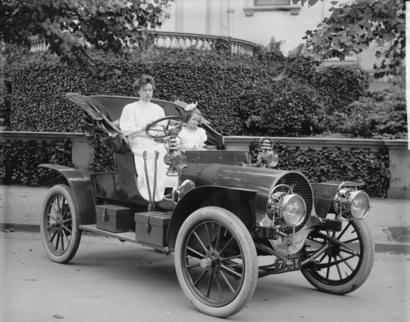
\includegraphics[width=\linewidth]{sample-franklin}
  \caption{1907 Franklin Model D roadster. Photograph by Harris \&
    Ewing, Inc. [Public domain], via Wikimedia
    Commons. (\url{https://goo.gl/VLCRBB}).}
  \Description{A woman and a girl in white dresses sit in an open car.}
\end{figure}

Your figures should contain a caption which describes the figure to
the reader.

Figure captions are placed {\itshape below} the figure.

Every figure should also have a figure description unless it is purely
decorative. These descriptions convey what’s in the image to someone
who cannot see it. They are also used by search engine crawlers for
indexing images, and when images cannot be loaded.

A figure description must be unformatted plain text less than 2000
characters long (including spaces).  {\bfseries Figure descriptions
  should not repeat the figure caption – their purpose is to capture
  important information that is not already provided in the caption or
  the main text of the paper.} For figures that convey important and
complex new information, a short text description may not be
adequate. More complex alternative descriptions can be placed in an
appendix and referenced in a short figure description. For example,
provide a data table capturing the information in a bar chart, or a
structured list representing a graph.  For additional information
regarding how best to write figure descriptions and why doing this is
so important, please see
\url{https://www.acm.org/publications/taps/describing-figures/}.

\subsection{Tables}

The ``\verb|acmart|'' document class includes the ``\verb|booktabs|''
package --- \url{https://ctan.org/pkg/booktabs} --- for preparing
high-quality tables.

Table captions are placed {\itshape above} the table.

Because tables cannot be split across pages, the best placement for
them is typically the top of the page nearest their initial cite.  To
ensure this proper ``floating'' placement of tables, use the
environment \textbf{table} to enclose the table's contents and the
table caption.  The contents of the table itself must go in the
\textbf{tabular} environment, to be aligned properly in rows and
columns, with the desired horizontal and vertical rules.  Again,
detailed instructions on \textbf{tabular} material are found in the
\textit{\LaTeX\ User's Guide}.

Immediately following this sentence is the point at which
Table~\ref{tab:freq} is included in the input file; compare the
placement of the table here with the table in the printed output of
this document.

\begin{table}
  \caption{Frequency of Special Characters}
  \label{tab:freq}
  \begin{tabular}{ccl}
    \toprule
    Non-English or Math&Frequency&Comments\\
    \midrule
    \O & 1 in 1,000& For Swedish names\\
    $\pi$ & 1 in 5& Common in math\\
    \$ & 4 in 5 & Used in business\\
    $\Psi^2_1$ & 1 in 40,000& Unexplained usage\\
  \bottomrule
\end{tabular}
\end{table}

To set a wider table, which takes up the whole width of the page's
live area, use the environment \textbf{table*} to enclose the table's
contents and the table caption.  As with a single-column table, this
wide table will ``float'' to a location deemed more
desirable. Immediately following this sentence is the point at which
Table~\ref{tab:commands} is included in the input file; again, it is
instructive to compare the placement of the table here with the table
in the printed output of this document.

\begin{table*}
  \caption{Some Typical Commands}
  \label{tab:commands}
  \begin{tabular}{ccl}
    \toprule
    Command &A Number & Comments\\
    \midrule
    \texttt{{\char'134}author} & 100& Author \\
    \texttt{{\char'134}table}& 300 & For tables\\
    \texttt{{\char'134}table*}& 400& For wider tables\\
    \bottomrule
  \end{tabular}
\end{table*}

Always use midrule to separate table header rows from data rows, and
use it only for this purpose. This enables assistive technologies to
recognise table headers and support their users in navigating tables
more easily.

\section{Citations and Bibliographies}

The use of BibTeX for the preparation and formatting of one's
references is strongly recommended. Authors' names should be complete
--- use full first names (``Donald E. Knuth'') not initials
(``D. E. Knuth'') --- and the salient identifying features of a
reference should be included: title, year, volume, number, pages,
article DOI, etc.

The bibliography is included in your source document with these two
commands, placed just before the \verb|\end{document}| command:
\begin{verbatim}
  \bibliographystyle{ACM-Reference-Format}
  \bibliography{bibfile}
\end{verbatim}
where ``\verb|bibfile|'' is the name, without the ``\verb|.bib|''
suffix, of the BibTeX file.

Citations and references are numbered by default. A small number of
ACM publications have citations and references formatted in the
``author year'' style; for these exceptions, please include this
command in the {\bfseries preamble} (before the command
``\verb|\begin{document}|'') of your \LaTeX\ source:
\begin{verbatim}
  \citestyle{acmauthoryear}
\end{verbatim}

  Some examples.  A paginated journal article \cite{Abril07}, an
  enumerated journal article \cite{Cohen07}, a reference to an entire
  issue \cite{JCohen96}, a monograph (whole book) \cite{Kosiur01}, a
  monograph/whole book in a series (see 2a in spec. document)
  \cite{Harel79}, a divisible-book such as an anthology or compilation
  \cite{Editor00} followed by the same example, however we only output
  the series if the volume number is given \cite{Editor00a} (so
  Editor00a's series should NOT be present since it has no vol. no.),
  a chapter in a divisible book \cite{Spector90}, a chapter in a
  divisible book in a series \cite{Douglass98}, a multi-volume work as
  book \cite{Knuth97}, a couple of articles in a proceedings (of a
  conference, symposium, workshop for example) (paginated proceedings
  article) \cite{Andler79, Hagerup1993}, a proceedings article with
  all possible elements \cite{Smith10}, an example of an enumerated
  proceedings article \cite{VanGundy07}, an informally published work
  \cite{Harel78}, a couple of preprints \cite{Bornmann2019,
    AnzarootPBM14}, a doctoral dissertation \cite{Clarkson85}, a
  master's thesis: \cite{anisi03}, an online document / world wide web
  resource \cite{Thornburg01, Ablamowicz07, Poker06}, a video game
  (Case 1) \cite{Obama08} and (Case 2) \cite{Novak03} and \cite{Lee05}
  and (Case 3) a patent \cite{JoeScientist001}, work accepted for
  publication \cite{rous08}, 'YYYYb'-test for prolific author
  \cite{SaeediMEJ10} and \cite{SaeediJETC10}. Other cites might
  contain 'duplicate' DOI and URLs (some SIAM articles)
  \cite{Kirschmer:2010:AEI:1958016.1958018}. Boris / Barbara Beeton:
  multi-volume works as books \cite{MR781536} and \cite{MR781537}. A
  couple of citations with DOIs:
  \cite{2004:ITE:1009386.1010128,Kirschmer:2010:AEI:1958016.1958018}. Online
  citations: \cite{TUGInstmem, Thornburg01, CTANacmart}. Artifacts:
  \cite{R} and \cite{UMassCitations}.
  
  If you want to include the author of some article you can use: ``\verb|\citeauthor|''. For example: \citeauthor{Knuth97} wrote a very famous book.
%%
%% The next two lines define the bibliography style to be used, and
%% the bibliography file.
\bibliographystyle{ACM-Reference-Format}
\bibliography{sample-base}

\end{document}
\endinput
%%
%% End of file `sample-authordraft.tex'.
